\subsection{Granular-Ball Consistency and Explained-Variation Dependency}
\label{subsec:ldl-dependency}
This subsection formalizes the attribute-induced granular representation for label distribution learning (LDL) and develops a support-constrained dependency metric based on explained variance. To prevent trivial interpolation while capturing genuine distributional separation, the formulation decouples intra-ball label consistency from inter-ball discrimination under explicit minimum-support constraints.

\subsubsection{Attribute-Induced Granular Representation}
Let $O = \{o_1, \dots, o_n\}$ denote the training instance set. For each attribute subset $P \subseteq A$, a deterministic granulation rule partitions $O$ into a set of mutually disjoint, nonempty granular balls $\mathcal{B}_P$. In this setting, the attribute space is governed by the directed dissimilarity defined in Section~\ref{subsec:ldl-directed} rather than a metric. Accordingly, a granular ball $B \in \mathcal{B}_P$ is characterized by a triple: its member set $B$, a medoid representative $c_P(B)$, and a radius descriptor $r_P(B)$.

The representative $c_P(B)$ is chosen as the medoid minimizing aggregate symmetric dissimilarity:
\begin{equation}
	c_P(B) = \underset{o \in B}{\operatorname{argmin}} \sum_{o' \in B} d_P(o, o'), \qquad
	d_P(o, o') = \max\left\{\overrightarrow{\rho}_P(o, o'), \overrightarrow{\rho}_P(o', o)\right\},
	\label{eq:medoid-selection}
\end{equation}
where ties are deterministically resolved by the canonical index ordering of $O$. Although $d_P$ does not necessarily satisfy the triangle inequality, it preserves the information-weighted directed deviations in both directions. The directional radii and the combined radius are given by
\begin{align}
	r_P^{\to}(B) &= \max_{o \in B} \overrightarrow{\rho}_P(c_P(B), o), \qquad
	r_P^{\leftarrow}(B) = \max_{o \in B} \overrightarrow{\rho}_P(o, c_P(B)), \\
	r_P(B) &= \max\left\{r_P^{\to}(B), r_P^{\leftarrow}(B)\right\}.
\end{align}
By convention, setting $P = \varnothing$ yields the trivial partition $\mathcal{B}_\varnothing = \{O\}$. Furthermore, instances that are identical across all selected attributes $P$ are treated as an indivisible unit; label distributions alone cannot fracture attribute-indistinguishable instances.

\subsubsection{Distribution Center, Dispersion, and Consistency}
Let $q = |Y|$ be the number of labels, $n_B = |B|$ the ball cardinality, and $\boldsymbol{p} = \bar{\boldsymbol{\ell}} = \frac{1}{n}\sum_{i=1}^n \boldsymbol{\ell}_i$ the global mean label distribution across the training set. For any ball $B$, we define its label distribution center $\boldsymbol{\mu}_B$ and within-ball dispersion $V(B)$ as
\begin{align}
	\boldsymbol{\mu}_B &= \frac{1}{n_B}\sum_{o_i \in B}\boldsymbol{\ell}_i, \label{eq:ball-label-center} \\
	V(B) &= \frac{1}{n_B}\sum_{o_i \in B} \|\boldsymbol{\ell}_i - \boldsymbol{\mu}_B\|_2^2, \qquad C(B) = 1 - V(B). \label{eq:ball-label-dispersion}
\end{align}
Since each $\boldsymbol{\ell}_i \in \Delta^{q-1}$ resides on the probability simplex, the center $\boldsymbol{\mu}_B$ is also a valid probability vector. The squared Euclidean loss in label space ensures an exact ANOVA-style variance decomposition.

\begin{proposition}[Properties of Label Dispersion]
	\label{prop:consistency-properties}
	For any granular ball $B$, the dispersion satisfies $0 \le V(B) \le 1 - 1/q$, and the consistency score satisfies $1/q \le C(B) \le 1$. Specifically:
\begin{enumerate}[label=(\roman*)]
		\item $C(B) = 1$ (or $V(B) = 0$) if and only if all instances in $B$ share an identical label distribution.
		\item If all $\boldsymbol{\ell}_i$ are degenerate one-hot distributions, $V(B)$ reduces to the standard empirical Gini impurity: $1 - \sum_{k=1}^q (\mu_B^k)^2$.
	\end{enumerate}
\end{proposition}
\begin{proof}
Expanding the squared distance around $\boldsymbol{\mu}_B$ yields
\[
V(B) = \frac{1}{n_B}\sum_{i \in B}\|\boldsymbol{\ell}_i\|_2^2 - \|\boldsymbol{\mu}_B\|_2^2.
\]

	Because $\boldsymbol{\ell}_i \in \Delta^{q-1}$, we have $\|\boldsymbol{\ell}_i\|_2^2 \le 1$. By the Cauchy--Schwarz inequality, $\|\boldsymbol{\mu}_B\|_2^2 \ge 1/q$. Hence, $0 \le V(B) \le 1 - 1/q$. The nonnegativity of squared norms implies that $V(B) = 0$ if and only if $\boldsymbol{\ell}_i = \boldsymbol{\mu}_B$ for all $o_i \in B$. When $\boldsymbol{\ell}_i$ are one-hot vectors, $\|\boldsymbol{\ell}_i\|_2^2 = 1$, which immediately yields the Gini impurity formulation.
\end{proof}

Proposition~\ref{prop:consistency-properties} highlights that dispersion measures distribution heterogeneity rather than informational entropy: a high-entropy but identical distribution (e.g., uniform $\boldsymbol{\ell}_i = (1/q, \dots, 1/q)$) achieves perfect consistency ($V(B) = 0$).

To set an adaptive consistency threshold, compute the global label dispersion
\begin{equation}
	V_0 = \frac{1}{n}\sum_{i=1}^n \|\boldsymbol{\ell}_i - \boldsymbol{p}\|_2^2.
	\label{eq:global-dispersion}
\end{equation}
Given a minimum support $s_{\min} \ge 2$, a radius bound $\alpha \in [0, 1]$, and a relative tolerance $\kappa \in [0, 1)$, we define the relative consistency threshold as $\delta = \kappa V_0$. Both $V_0$ and $\delta$ are determined strictly on the training partition. A ball $B$ is termed \emph{eligible} if it jointly satisfies support, consistency, and compactness constraints:
\begin{equation}
	\mathcal{E}_P = \left\{ B \in \mathcal{B}_P : n_B \ge s_{\min}, \ V(B) \le \delta, \ r_P(B) \le \alpha \right\}.
	\label{eq:eligible-balls}
\end{equation}
The condition $s_{\min} \ge 2$ explicitly excludes singletons from $\mathcal{E}_P$, preventing trivial overfitting through pure interpolation.

\subsubsection{Dependency as Explained Label Distribution Variation}
To evaluate the representative capacity of $\mathcal{B}_P$, instances belonging to eligible balls are represented by their local centers $\boldsymbol{\mu}_B$, whereas instances in ineligible balls fall back to the global prior $\boldsymbol{p}$. The resulting training reconstruction error is
\begin{equation}
	R(P) = \frac{1}{n} \left[
	\sum_{B \in \mathcal{E}_P} \sum_{i \in B} \|\boldsymbol{\ell}_i - \boldsymbol{\mu}_B\|_2^2 +
	\sum_{B \in \mathcal{B}_P \setminus \mathcal{E}_P} \sum_{i \in B} \|\boldsymbol{\ell}_i - \boldsymbol{p}\|_2^2
	\right].
\end{equation}

\begin{definition}[Support-Constrained LDL Dependency]
	\label{def:ldl-dependency}
	The granular-ball dependency of attribute subset $P$ is defined as the fraction of global label variance explained by the eligible balls:
	\begin{equation}
		\Gamma(P) =
		\begin{cases}
			1 - \dfrac{R(P)}{V_0} = \dfrac{\sum_{B \in \mathcal{E}_P} n_B \|\boldsymbol{\mu}_B - \boldsymbol{p}\|_2^2}{n V_0}, & V_0 > 0, \\[8pt]
			0, & V_0 = 0.
		\end{cases}
		\label{eq:ldl-explained-dependency}
	\end{equation}
\end{definition}

\begin{proposition}[Variance Decomposition and Boundedness]
	\label{prop:variance-bounds}
	For any attribute subset $P \subseteq A$, $0 \le \Gamma(P) \le 1$ and $\Gamma(\varnothing) = 0$. Specifically:
\begin{enumerate}[label=(\roman*)]
		\item $\Gamma(P) = 0$ if and only if either $\mathcal{E}_P = \varnothing$ or $\boldsymbol{\mu}_B = \boldsymbol{p}$ for all $B \in \mathcal{E}_P$.
		\item $\Gamma(P) = 1$ if and only if all instances belong to eligible balls, each eligible ball has zero dispersion ($V(B)=0$), and every instance in any remaining ineligible ball carries exactly the global prior $\boldsymbol{p}$.
	\end{enumerate}
\end{proposition}
\begin{proof}
	Because $\sum_{i \in B}(\boldsymbol{\ell}_i - \boldsymbol{\mu}_B) = \mathbf{0}$, the cross-term vanishes, providing an orthogonal sum-of-squares decomposition for each ball $B$:
	\begin{equation}
		\sum_{i \in B} \|\boldsymbol{\ell}_i - \boldsymbol{p}\|_2^2 = n_B V(B) + n_B \|\boldsymbol{\mu}_B - \boldsymbol{p}\|_2^2.
		\label{eq:ball-variance-decomposition}
	\end{equation}
	Summing over all $B \in \mathcal{B}_P$ and subtracting $n R(P)$ from $n V_0$ cancels the intra-ball dispersion terms for eligible balls, leaving exactly the numerator in Eq.~\eqref{eq:ldl-explained-dependency}. Since $0 \le R(P) \le V_0$, the bounds follow immediately.
\end{proof}

\subsubsection{Monotonicity Non-Preservation and Non-Convexity}
A critical property of $\Gamma(P)$ is that it does not generally satisfy subset monotonicity, i.e., $P \subseteq Q \not\implies \Gamma(P) \le \Gamma(Q)$. 
Although the unconstrained between-group variation $\sum_{B \in \mathcal{B}_P} n_B \|\boldsymbol{\mu}_B - \boldsymbol{p}\|_2^2$ increases monotonically under nested partition refinements, the support constraint ($n_B \ge s_{\min}$) creates a combinatorial threshold:
\begin{itemize}
	\item A refined partition may shatter a valid eligible ball into sub-balls with cardinalities below $s_{\min}$, converting an eligible contribution into an ineligible fallback.
	\item Transitioning from $P$ to $Q$ reconstructs the entire metric space, shifting representative medoids and ball boundaries non-locally.
\end{itemize}
Consequently, attribute selection guided by $\Gamma(P)$ requires search procedures capable of handling non-monotonic objective landscapes.

\subsection{Deterministic Granular-Ball Construction}
\label{subsec:granulation-rule}
To materialize the partition $\mathcal{B}_P$ deterministically, we provide a top-down, supervised binary granulation procedure. 

\subsubsection{Attribute Atoms and Seed-Pair Partitioning}
To preserve attribute indistinguishability, instances sharing identical feature projections on $P$ are grouped into an \emph{attribute atom} $G \subseteq B$. Each atom is treated as an indivisible entity and indexed by its lowest-index instance $u_G$. Let $\mathcal{A}_P(B)$ denote the set of atoms within $B$. 

If $|\mathcal{A}_P(B)| \ge 2$, two distinct seed atoms $(u, v)$ are identified by maximizing the mutual symmetric dissimilarity:
\begin{equation}
	(u, v) = \underset{u_G, u_H:\, G \ne H}{\operatorname{argmax}} d_P(u_G, u_H), \quad \text{subject to } u < v,
	\label{eq:granular-seeds}
\end{equation}
with ties resolved by lexicographical index order. All atoms in $B$ are then assigned to the nearer seed:
\begin{equation}
	B_1 = \bigcup_{G:\, d_P(u_G, u) \le d_P(u_G, v)} G, \qquad B_2 = B \setminus B_1.
	\label{eq:atom-assignment}
\end{equation}
Tied distances are assigned to the primary seed $u$.

\subsubsection{Admissibility and Stopping Criteria}
A prospective split $(B \to B_1, B_2)$ is accepted if and only if it satisfies both structural feasibility and progressive improvement:
\begin{enumerate}
	\item \textbf{Support admissibility:} $\min\{n_{B_1}, n_{B_2}\} \ge s_{\min}$.
	\item \textbf{Progressive gain:} The candidate achieves a minimal reduction in either label dispersion or geometric radius:
	\begin{equation}
		g_V(B; B_1, B_2) > \varepsilon_V \quad \text{or} \quad g_r(B; B_1, B_2) > \varepsilon_r,
		\label{eq:split-improvement}
	\end{equation}
	where the variance gain is defined as:
\begin{equation}
	\begin{split}
		g_V(B; B_1, B_2) &= V(B) - \frac{n_{B_1}V(B_1) + n_{B_2}V(B_2)}{n_B} \\
		&= \frac{n_{B_1}\|\boldsymbol{\mu}_{B_1} - \boldsymbol{\mu}_B\|_2^2 + n_{B_2}\|\boldsymbol{\mu}_{B_2} - \boldsymbol{\mu}_B\|_2^2}{n_B} \ge 0,
	\end{split}
\end{equation}

	and the radius contraction gain is $g_r = r_P(B) - \max\{r_P(B_1), r_P(B_2)\}$.
\end{enumerate}
If a ball is eligible ($B \in \mathcal{E}_P$), contains fewer than $2s_{\min}$ instances, or fails both gain thresholds, it becomes a terminal leaf. The overall procedure is summarized in Algorithm~\ref{alg1:reference-granulation}; Figure~\ref{fig:granulation-neggain} illustrates how the induced ball structure and its dependency can change non-monotonically when the attribute subset grows, which is the structural reason dependency gains must be treated as signed quantities.

\begin{figure}[htbp]\centering
	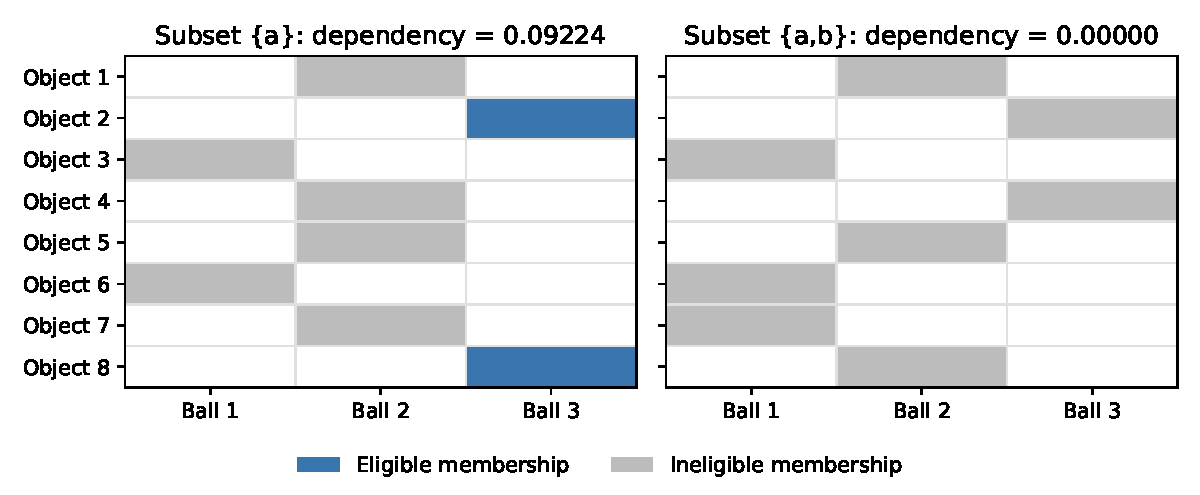
\includegraphics[width=.92\linewidth]{granulation_negative_gain.pdf}
	\caption{Non-monotone granulation on a synthetic eight-object construction: adding attribute $b$ to subset $\{a\}$ reshapes the ball partition (objects re-assigned across balls, eligibility changes) and can \emph{lower} the granular dependency despite distance monotonicity. Shading distinguishes eligible from ineligible ball membership.}
	\label{fig:granulation-neggain}
\end{figure}

\begin{algorithm}[t]
	\caption{Deterministic Granular-Ball Partitioning for Subset $P$}
	\label{alg1:reference-granulation}
	\begin{algorithmic}[1]
		\Require Training set $O$, attribute subset $P$, parameters $(s_{\min}, \kappa, \alpha, \varepsilon_V, \varepsilon_r)$
		\Ensure Granular partition $\mathcal{B}_P$, eligible ball set $\mathcal{E}_P$, dependency $\Gamma(P)$
		\State Compute $V_0$ via Eq.~\eqref{eq:global-dispersion} and set $\delta \gets \kappa V_0$
		\State Initialize empty leaf set $\mathcal{B}_P \gets \emptyset$, queue $\mathcal{Q} \gets \{O\}$
		\While{$\mathcal{Q} \ne \emptyset$}
		\State Dequeue current member set $B \gets \operatorname{pop}(\mathcal{Q})$
		\If{$B \in \mathcal{E}_P$ \textbf{or} $n_B < 2s_{\min}$}
		\State $\mathcal{B}_P \gets \mathcal{B}_P \cup \{B\}$; \textbf{continue}
		\EndIf
		\State Form attribute atoms $\mathcal{A}_P(B)$
		\If{$|\mathcal{A}_P(B)| < 2$ \textbf{or} $\max_{G \ne H} d_P(u_G, u_H) = 0$}
		\State $\mathcal{B}_P \gets \mathcal{B}_P \cup \{B\}$; \textbf{continue}
		\EndIf
		\State Find seed pair $(u, v)$ via Eq.~\eqref{eq:granular-seeds} and split into $(B_1, B_2)$ via Eq.~\eqref{eq:atom-assignment}
		\If{$\min\{n_{B_1}, n_{B_2}\} \ge s_{\min}$ \textbf{and} ($g_V > \varepsilon_V$ \textbf{or} $g_r > \varepsilon_r$)}
		\State Enqueue $\mathcal{Q} \gets \operatorname{push}(\mathcal{Q}, B_1, B_2)$
		\Else
		\State $\mathcal{B}_P \gets \mathcal{B}_P \cup \{B\}$
		\EndIf
		\EndWhile
		\State Extract $\mathcal{E}_P \gets \{B \in \mathcal{B}_P : V(B) \le \delta \land r_P(B) \le \alpha\}$
		\State Compute $\Gamma(P)$ via Eq.~\eqref{eq:ldl-explained-dependency}
		\State \Return $\mathcal{B}_P$, $\mathcal{E}_P$, $\Gamma(P)$
	\end{algorithmic}
\end{algorithm}

\begin{proposition}[Termination and Determinism]
	Algorithm~\ref{alg1:reference-granulation} terminates in at most $\lfloor n/s_{\min} \rfloor - 1$ splits, outputting a disjoint partition of $O$ that preserves attribute atoms.
\end{proposition}
\begin{proof}
	Each accepted split generates two disjoint subsets of size at least $s_{\min}$. Thus, the number of leaves $L$ satisfies $L s_{\min} \le n$, which bounds the split operations by $\lfloor n/s_{\min} \rfloor - 1$. Determinism follows directly from the invariant tie-breaking rules on instance indices and the deterministic FIFO queue processing.
\end{proof}

\subsubsection{Computational Complexity and Practical Overhead}
With pairwise attribute distances precomputed, evaluating $d_P$ costs $O(n^2 |P|)$. For a node of size $b$, identifying seed atoms and medoids requires $O(b^2)$ operations, and computing label dispersion costs $O(bq)$. In the worst-case unbalanced tree, the cumulative granulation cost per subset evaluation is bounded by $O(n^3 + n^2 q)$. Under typical balanced splits, the time complexity scales closer to $O(n^2 \log(n/s_{\min}))$.